\section{Applications for Large Models}
\label{sec:applications}

In this section, we look at examples for three modeling applications. We do this for two reasons. The first reason is to discuss the actual practical relevance of large models. The second reason is to identify model usage patterns: which of the four modeling tasks (create, traverse, query, partial load) are actually used, in what frequency, and with what parameters. At the end of this section, we provide a tabular summary of our assessment.

%The first one is software modeling, which is what most of the MODELS community is concerned with and what the modeling frameworks mentioned in this paper were designed for. But techniques originally developed for software modeling are also used for other applications. More abstractly, software modeling can be explained as the representation, analysis, and manipulation of structured data. 
%
%Our research group, for example, uses EMF to represent and analyse sensor data received from our wireless sensor network test-bed (\emph{Humboldt Wireless Lab}~\cite{hwl}). Models of heterogeneous sensor data will be our second application. 
%This application is what actually motivated us as authors for this work, because existing approaches where either impractical (lazy loading of EMF resources), or far to slow to store the data at the rate it was produced (CDO and manual relational data base persistence). 
%Refer to~\cite{clickwatch} for more details. 
%
%The third application that we want to analyse, are geo-spatial models and more specifically 3D object models of cities. Such models represent the features of a city (boroughs, streets, buildings, floors, rooms, windows, etc.) as a containment hierarchy of objects and their properties. 
%These models are closely related to sensor data analysis.
%
%For all three applications, we estimate the size of typical models. Furthermore, we determine the most important use cases for all three applications. From these use cases we derive the commonly used modeling tasks and their characteristics.

\subsection{Software Models}
Model Driven Software Development (MDSD) is the application that modelling frameworks like EMF were actually designed for. In MDSD all artifacts including traditional software models as well as software code are understood as models~cite{modelsAsCode}, i.e. directed labelled graphs of typed nodes with an inherent containment hierarchy. 
%IDEs (e.g. eclipse's JDT or CDT) already represent code as models (ASTs). Advances in modeling frameworks (e.g. model comparison) suggests that code is also persisted as model.

\subsubsection*{Model Size}

Since models of software code (code models) provide the lowest level of abstraction, we assume that models of software code are the largest software models. Therefore, software projects with a large code base probably provide the largest examples for software models. We will first look at the Linux Kernel as an example for a large software project and then extend our estimates on other operating system projects.

Traditionally code size is measured in \emph{lines of code} LOC (physical lines), SLOC (source LOC, like LOC but without empty lines, comments, duplicates), and LLOC (logical LOC, like SLOC but normalized to one statement per line).~\cite{wheeler} 
These measures exist for many known software projects (and their history) and can be easily captured for open source projects. 

To estimate the size of code models in number of objects, we additionally need to know how many model objects constitute an average LOC. We used the C Development Toolkit (CDT) to parse the current version of the Linux Kernel (3.2.1) and count the number of abstract syntax tree (AST) nodes required. We assume that model objects and AST nodes are equivalent for our estimation. We also counted the LOCs of the Kernel's code with \emph{sloccount}. This provides an model objects per LOC ratio of 5.99 that we use for all further estimates.

From the GIT versioning system we learned the average numbers of added, removed, and manipulated LOCs per month based on last year's history (4,300 LOC added, 1,800 LOC removed, and 1,500 LOC modified per day). We extrapolate these numbers to estimate the older history of the Kernel. Based on the actual grow in LOC over the last years and our model objects per LOC ratio, we calculated the average number of modified objects in a modified LOC, and can finally estimates the number of all objects in the Kernel's code including its history. This is a model that only contains the changes.

\begin{figure}
  \centering
  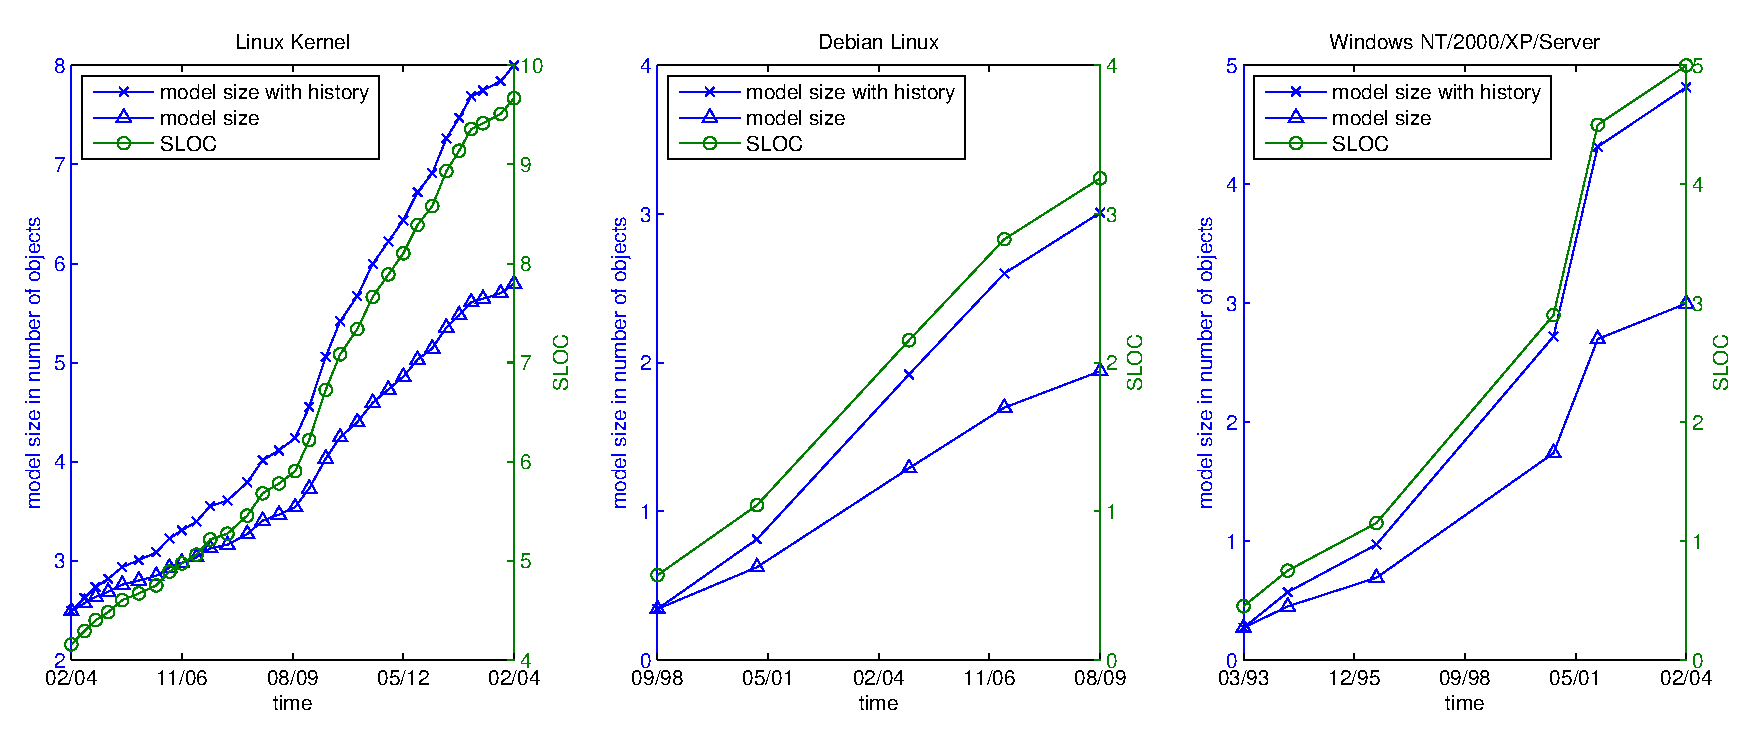
\includegraphics[width=\linewidth]{figures/software_model_sizes}
  \caption{Rough estimates for software code model sizes based on actual SLOC counts for existing software projects.}
  \label{fig:software_model_sizes}
\end{figure}


We also transferred all ratios from the Kernel to other OS software projects and publicly reported LOC counts. The results represent rough estimates and are presented in Fig.~\ref{fig:software_model_sizes}. As you can see, these large software models can have a size upto a magnitude of $10^9$ objects.

Furthermore, it is not clear whether further growth in software project size is exponential or linear. Some believe that software size follows Moore's Law. Others think that software is bound by increasing complexity and not by the limitations of underlying hardware.

\subsubsection*{Usage Patterns}
There are two major use cases in today's software development: editing and transforming or compiling. The first use case is either performed on diagrams (graphical editing) or on compilation units (e.g. Java-files, textual editing). Diagram contents roughly corresponds to package contents. Both packages and compilation units are sub-trees within the containment tree of a software model.  Transformations or compilations are usually either done for the whole model or again on a per package or compilation unit basis. Within these aggregates, the (partial) model is traversed. A further use-case is analysis. Analysis is sometimes performed with single queries. But due to performance issues, model analysis is more often performed by traversing the model and by executing multiple queries with techniques similar to model transformations. Software models are only accessed by a view individuals at the same time.

%\subsubsection{What are software code models?}
%We use the term model to describe MDSD artifacts. Originally these artifacts were models on a high level of abstraction, but today programming code, can also be understood as models. For example IDEs such as eclipse JDT or eclipse CDT internally maintain programming code as ASTs (primitive models) in order to provide advanced IDE features such as outlines, error annotations, type and call hierarchies, and code completion. It is safe to assume that programming code contains far more information compared to high-level models. Since we are looking for extra large models, we will concentrate on software code models.
%
%Advances in language workbenches suggest to replace these IDEs with eclipse EMF based and generated tools. Advances in comparison and versioning of models will soon allow to replace per-line-text-file-based versioning systems (e.g. CSV, SVN, GIT) with model based (e.g. EMF-based) systems that version on a per mode-object- or even per-object-attribute basis.
%
%\subsubsection{How big is are existing software code models?}
%How large are these software code models? Traditionally code size is measured in \emph{lines of code} LOC (physical lines), SLOC (source LOC, like LOC but without empty lines, comments, duplicates; refer to Wheeler~\cite{wheeler}, and LLOC (logical LOC, like SLOC but normalized to one statement per line). These measures exist for many known software projects (and their history) and can be easily captured for open source projects. 
%
%In order to determine corresponding model sizes, we need to know how much model objects each LOC represents. To estimate this, we used the eclipse CDT parser as tool and the linux kernel as sample. The CDT parser is specialized to parse C/C++ code in its un-preprocessed form. Thus, the resulting ASTs are not bloated with information injected (with lots of duplicates) during pre-processing. Of course ASTs are not software models as they are understood in the OMG/EMF world, but we can assume that proper C/C++ models will contain one object for each AST node. \markus{This needs a reference}. Parsing the current kernel version, counting its AST nodes, and comparing this number to the kernel's SLOC number gives us a good estimate for objects per SLOC (at least for the kernel code, probably for all C code, and maybe it is also a good estimate for other similar programming languages, e.g. C\#, Java). We will use this estimate to extrapolate the model size of other kernel versions and other software projects. 
%
%Eventually, we want to store software models and its versions. Of course, we only want to store the differences between versions. A software projects model size is determined by the size of the differences that produced the current software model. To determine this size, we need to know how much LOCs were added, removed, and modified in a software project. To estimate this, we use the versioning system GIT as tool and the linux kernel GIT repository as sample. With gitstats we can determine the number of added, removed, and changed lines throughout the repository history. With these numbers, the estimated objects per SLOC and the recorded SLOCs for different kernel versions we can estimate the model size of a kernel software code model repository. We can also assume that other software projects have a similar proportion of added, removed, and modified lines, and transfer these estimates to other software projects. 
%
%\begin{figure}
%  \centering
%  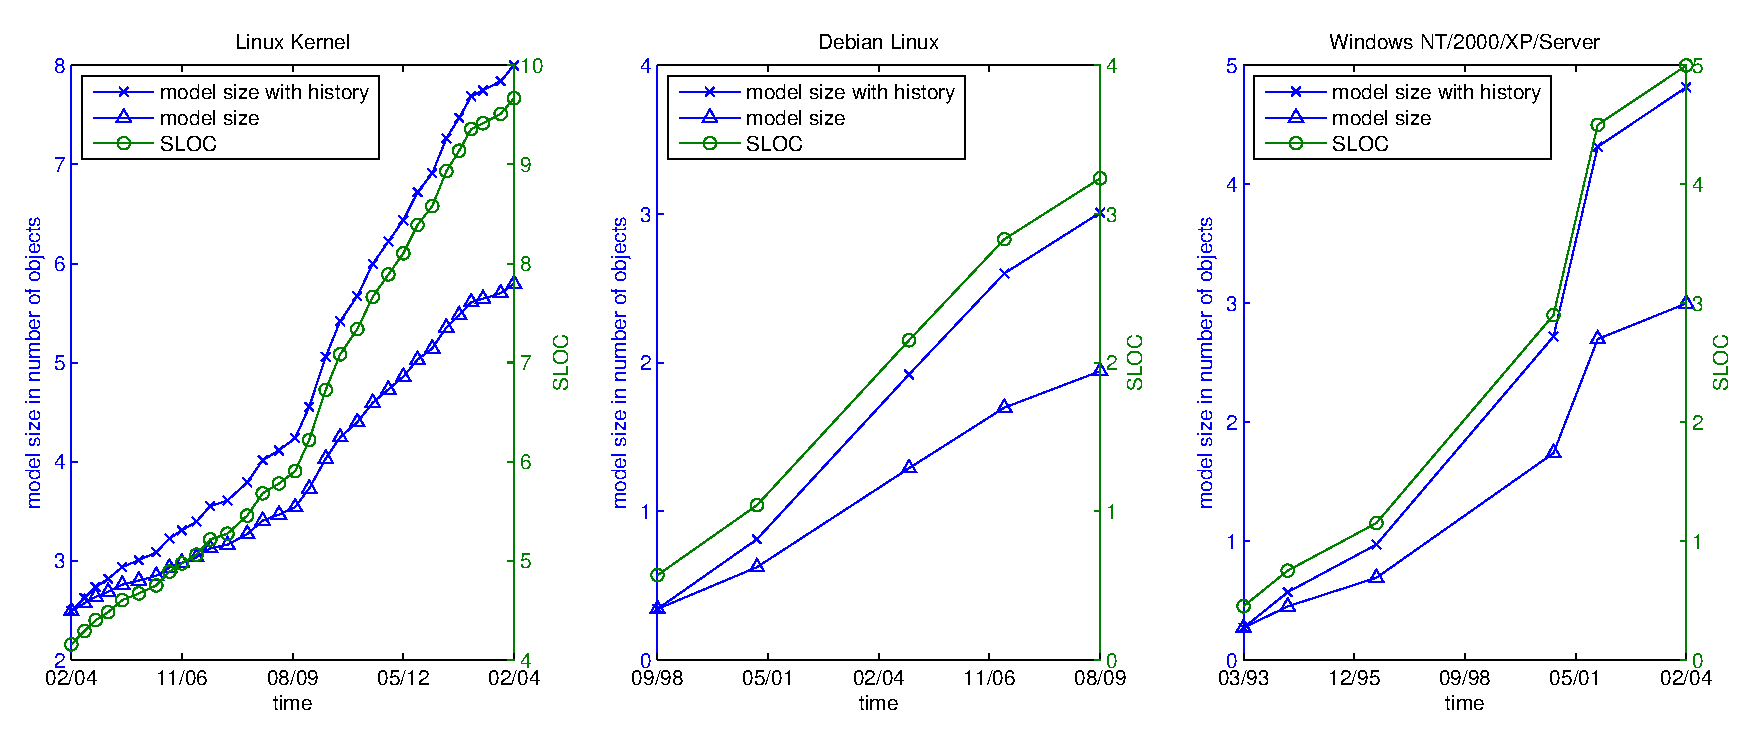
\includegraphics[width=\linewidth]{figures/software_model_sizes}
%  \caption{SLOC and estimated number of objects for popular large software projects.}
%  \label{fig:software_model_sizes}
%\end{figure}
%
%Fig.~\ref{fig:software_model_sizes} shows the LOC numbers and estimated object numbers in corresponding software code models. The charts present different software projects and how size developed over time. \markus{kernel, linux(debian)?, windows - numbers based on kernel git alone, SLOC numbers and transferred kernel estimates.}
%
%\subsubsection{How big are software code models in the future?}
%
%Some believe that the average size software (and software code models for that matter) grows faster than linear following Moore's Law. Maciej Soltysiak for example has analysed the grows of the linux kernel code base and observed exponential growth. A counter argument is that software not only bound by hardware limitations (i.e. Moore's Law) but increasingly by software complexity and therefore will not grow exponentially. Never the less, it is safe to assume that software code models will be larger in the future.

\subsection{Heterogenous Sensor Data}

Sensor data usually comprises of time series of measured physical values in the environment of a sensor; but sensor data can also contain patterns of values (e.g. video images). Sensor data is collected in sensor networks, that combine distributes sensors with an communication infrastructure. Sensor data can be heterogeneous: a sensor network can use different types of sensors that measure a multitude of parameters. \cite{estrin,lynch}. 

Our research group build the \emph{Humboldt Wireless Lab}~\cite{hwl}, a 120 node wireless sensor network. Nodes are equipped with 3 axis accelerometers, but more essentially also produce data from monitoring all running software components (mostly networking protocols), and other system parameters (eg.g. CPU, memory, or radio statistics). We represent and analyse this data as EMF based models (\cite{clickwatch}).
% add cites for SMTL once accepted

\subsubsection*{Model Size}
HWL's network protocols and system software components provide 372 different types of data sets. Each data set is represented as an XML document. Per second each node in the network produces XML entities that translate into an average of 1120 EMF objects. A common experiment with HWL involves 50 nodes and measures of a period of 24h. During such an experiment, the network produces a model of $5*10^9$ objects. 

In general, sensor networks are only bounded by the limitations of the technical infrastructure that supports them. Ambiguous computing and Smart Citys suggest future sensor data models of arbitrary sizes. 

\subsubsection*{Usage Patterns}
There are two major use-cases: recording sensor data and analysing sensor data. Recording sensor data means to store it faster then it is produced. If possible in a manner that supports later analysis. Sensor data is rarely manipulated. Analysis means to access and traverse individual data sets (mostly time series). Each data set or recorded set of data sets is a sub-tree in the sensor data model. Recording and analysis is usually performed by only a single (or a few) individuals at the same time. 

\subsection{Geospatial Models}

3D city models are a good example for structured geo-spatial information. The CityGML~\cite{cityGML} standard, provides a set of xml-schemas (building upon other standards, e.g. GML) that function as a meta-model. CityGML models represent the features of a city (boroughs, streets, buildings, floors, rooms, windows, etc.) as a containment hierarchy of objects. 
%These models are closely related to sensor data analysis.
%CityGML, compared to other quasi standards (e.g. google's KML) does not solely concentrate on 3D measures, but allows to extend the covered information by more semantic attributes (e.g. materials, age, inhabitants, existing infrastructure, etc.).
Geo spatial models usually come in different levels of details (LOD); CityGML distinguishes 5 LODs, 0-4)~\cite{cityGML}. 

\subsubsection{Model Size}
As for many cities, a CityGML model is currently established for berlin~\cite{berlinGML}. The current model of Berlin covers all of Berlin, but mostly on a low-medium level of detail (LOD 1-2). To get an approximation of the model's size, we counted the XML entities. The current Berlin model, contains roughly $128*10^6$ objects. 

Estimated on existing CityGML models published for Berlin~\cite{berlinGML} a LOD 1 building consists of 12.5 objects, a LOD 2 building of 40 objects, and a LOD 3 building of 350 objects. A complete LOD 3-4 model of Berlin would therefore consist of $1*10^9$ objects. Berlin inhabits 3.5 million people. About 50\% of the worlds $7*10^9$ people live in cities. This gives a whole LOD3-4 approximation of $10^{12}$ objects for a \emph{world 3D city model}.

\subsubsection{Usage Patterns}
Compared to model manipulation, model access is far more common and its efficient execution is paramount. If accessed, users usually load a containment hierarchies (sub-tree) corresponding to a given set of coordinates or address (geographic location): partial loads. Queries for distinct feature characteristics within a specific geographic location (i.e. with-in such a partial load) are also common. Geo-spatial models are accessed by many people at the same time. 

\subsection*{Summary\footnote{Plus and minus signs characterise the importance of time efficiency for the corresponding property or task from 0 to 3.}}
\begin{tabular}{|c||c|c|c|c|c|c|}
\hline
\bf{application} & \bf{model size} & \bf{parallel} & \bf{create} & \bf{traverse} & \bf{query} & \bf{part. load} \\
\hline\hline
software models & $0-10^9$ & - & - & ++ & + & ++ \\
\hline
sensor data & $10^9$ & - & +++ & ++ & - & ++ \\
\hline
geo-spatial models & $10^9-10^{12}$ & +++ & - & + & + & +++ \\
\hline
\end{tabular}



